\documentclass[12pt,a4paper, spanish]{article}
% Sacar draft para que aparezcan las imagenes.
% Opciones: 12pt, 10pt, 11pt, landscape, twocolumn, fleqn, leqno...
% Opciones de clase: article, report, letter, beamer...

% Paquetes:
% =========
\usepackage[headheight=110pt, top = 2cm, bottom = 2cm, left=1cm, right=1cm]{geometry} %modifico márgenes
\usepackage[T1]{fontenc} % tildes
\usepackage[utf8]{inputenc} % Para poder escribir con tildes en el editor.
\usepackage[english]{babel} % Para cortar las palabras en silabas, creo.
\usepackage[ddmmyyyy]{datetime}
\usepackage{amsmath} % Soporte de mathmatics
\usepackage{amssymb} % fuentes de mathmatics
\usepackage{array} % Para tablas y eso
\usepackage{caption} % Configuracion de figuras y tablas
\usepackage[dvipsnames]{xcolor} % Para colorear el texto: black, blue, brown, cyan, darkgray, gray, green, lightgray, lime, magenta, olive, orange, pink, purple, red, teal, violet, white, yellow.
\usepackage{graphicx} % Necesario para poner imagenes
\usepackage{enumitem} % Cambiar labels y más flexibilidad para el enumerate
\usepackage{multicol} 
\usepackage{tikz} % para graficar
\usepackage{cancel} % cancelar fórmulas
\usepackage{titlesec} % para editar titulos y hacer secciones con formato a medida
\usepackage{ulem}
\usepackage{centernot} % tacha cosas
\usepackage{bbding} % símbolos de donde uso FiveStar
\usepackage{skull} % símbolos de donde uso Skull
\usepackage{soul} % Para tachar texto en text y math mode

% \usepackage{lipsum} % dummy text

% para hacer los graficos tipo grafos
\usetikzlibrary{shapes,arrows.meta, chains, matrix, calc, trees, positioning, fit}
\usetikzlibrary{external}

\setlength{\parindent}{0pt} % Para que no haya indentación en las nuevas líneas.

% Definiciones y macros para que se me haga
% más ameno el codeo.
% Definiciones y nuevos comandos:def
% =============
% Conjuntos
\DeclareMathOperator{\partes}{\mathcal P}
\DeclareMathOperator{\relacion}{\,\mathcal{R}\,}
\DeclareMathOperator{\norelacion}{\,\cancel{\relacion}\,}
\DeclareMathOperator{\universo}{\mathcal U}
\DeclareMathOperator{\reales}{\mathbb R}
\DeclareMathOperator{\naturales}{\mathbb N}
\DeclareMathOperator{\enteros}{\mathbb Z}
\DeclareMathOperator{\racionales}{\mathbb Q}
\DeclareMathOperator{\irracionales}{\mathbb I}
\DeclareMathOperator{\complejos}{\mathbb C}


\DeclareMathOperator{\K}{\mathbb K} % cuerpo K
\DeclareMathOperator{\vacio}{\varnothing}
\DeclareMathOperator{\union}{\cup}
\DeclareMathOperator{\inter}{\cap}
\DeclareMathOperator{\diferencia}{\ \setminus \ }
\DeclareMathOperator{\y}{\land}
\def\o{\lor}
\def\neg{\sim}

\def\entonces{\Rightarrow}
\def\noEntonces{\centernot\Rightarrow}

\def\sisolosi{\iff} % largo
\def\sii{\Leftrightarrow} % corto

\def\clase{\overline}
\def\ord{\text{ord}}


\def\existe{\,\exists\,}
\def\noexiste{\,\nexists\,}
\def\paratodo{\ \, \forall}
\def\distinto{\neq}
\def\en{\in}
\def\talque{\;/\;}

% =====
\def\qvq{\text{ quiero ver que }}

%funciones
\DeclareMathOperator{\dom}{Dom}
\DeclareMathOperator{\cod}{Cod}
\def\F{\mathcal F}
\def\comp{\circ}
\def\inv{^{-1}}
\def\infinito{\infty}

% Llaves, paréntesis, contenedores
\newcommand{\llave}[2]{ \left\{ \begin{array}{#1} #2 \end{array}\right. }
\newcommand{\llaveInv}[2]{ \left\} \begin{array}{#1} #2 \end{array}\right. }
\newcommand{\llaves}[2]{ \left\{ \begin{array}{#1} #2 \end{array} \right\} }
\newcommand{\matriz}[2]{\left( \begin{array}{#1} #2 \end{array} \right)}
\newcommand{\deter}[2]{\left| \begin{array}{#1} #2 \end{array} \right|}
\newcommand{\lista}[2][(1)]{\begin{enumerate}[\bf #1]\setlength\itemsep{-0.6ex} #2 \end{enumerate}}
\newcommand{\listal}[2][-0.6ex]{\begin{enumerate}[\bf(a)]\setlength\itemsep{#1} #2 \end{enumerate}}

% naturales
\newcommand{\sumatoria}[2]{\sum\limits_{#1}^{#2}}
\newcommand{\productoria}[2]{\prod\limits_{#1}^{#2}}
\newcommand{\kmasuno}[1]{\underbrace{#1}_{k+1\text{-ésimo}}}
\newcommand{\HI}[1]{\underbrace{#1}_{\text{HI}}}

% % enteros
\def\divideA{\, | \,}
\def\noDivide{\centernot\divideA}
\def\congruente{\, \equiv \,}
\newcommand{\congruencia}[3]{#1 \equiv #2 \;(#3)}
\newcommand{\noCongruencia}[3]{#1 \not\equiv #2 \;(#3)}
\newcommand{\conga}[1]{\stackrel{(#1)}{\congruente}}
\newcommand{\divset}[2]{\mathcal{D}(#1) = \set{#2}}
\newcommand{\divsetP}[2]{\mathcal{D_+}(#1) = \set{#2}}
\newcommand{\ub}[2]{ \underbrace{\textstyle #1}_{\mathclap{#2}} }
\newcommand{\ob}[2]{ \overbrace{\textstyle #1}^{\mathclap{#2}} }
\def\cop{\, \perp \, }

% complejos
\DeclareMathOperator{\re}{Re}
\DeclareMathOperator{\im}{Im}
\DeclareMathOperator{\argumento}{arg}
\newcommand{\conj}[1]{\overline{#1}}

% Polinomios
\DeclareMathOperator{\cp}{cp}
\DeclareMathOperator{\gr}{gr}
\DeclareMathOperator{\mult}{mult}
\newcommand{\divPol}[2]{\polylongdiv[style=D]{#1}{#2}}
\newcommand{\mcd}[2]{\polylonggcd{#1}{#2}}


% =====
% Miscelanea
% =====
\def\ot{\leftarrow}
\newcommand{\estabien}{{\color{blue} Consultado, está bien. \checkmark}}
\newcommand{\hacer}{
  {\color{red!80!black}{\Large \faIcon{radiation} Falta hacerlo!}}\par
  {\color{black!70!white}
    \small Si querés mandarlo: Telegram $\to$ \href{https://t.me/+1znt2GV1i8cwMTNh}{\small\faIcon{telegram}},
    o  mejor aún si querés subirlo en \LaTeX $\to$ \href{https://github.com/nad-garraz/algebraUno}{\small \faIcon{github}}.
  }\par
}

\newcommand{\Hacer}{{\color{black!30!red}\Large Hacer!}}
\def\Tilde{\quad\checkmark}
\def\ytext{\text{ y }}
\def\otext{\text{ o }}

% Estrellita para hacer llamadas de atención, viene en divertidos colores
% para coleccionar.
\newcommand{\llamada}[1]{
  \textcolor{
    \ifcase \numexpr#1 mod 6\relax
      cyan\or magenta\or OliveGreen\or YellowOrange\or Cerulean\or Violet\or Purple\or
    \fi
  }
  {\text{\FiveStar}^{\scriptscriptstyle#1}}
}


% separadores
\def\separador{\par\medskip\rule{\linewidth}{0.4pt}\par\medskip}
\def\separadorCorto{\par\medskip\rule{0.5\linewidth}{0.4pt}\par\medskip}


% Colores
\newcommand{\red}[1]{\textcolor{red}{#1}}
\newcommand{\green}[1]{\textcolor{OliveGreen}{#1}}
\newcommand{\blue}[1]{\textcolor{Cerulean}{#1}}
\newcommand{\cyan}[1]{\textcolor{cyan}{#1}}
\newcommand{\yellow}[1]{\textcolor{YellowOrange}{#1}}
\newcommand{\magenta}[1]{\textcolor{magenta}{#1}}
\newcommand{\purple}[1]{\textcolor{purple}{#1}}

% Conjuntos entre llaves y paréntesis
% te ahorrás escribir los \left y \right, así dejando el código más legible.
\newcommand{\set}[1] { \left\{ #1 \right\} }
\newcommand{\parentesis}[1]{ \left( #1 \right) }

% Stackrel text. Es para ahorrarse ecribir el \text
\newcommand{\stacktext}[2]{ \stackrel{\text{#1}}{#2} }

% Dado que muchas veces ponemos cosas sobre un signo '='
%  acá está el comando para escribir \igual{arriba}[abajo] con texto!
\NewDocumentCommand{\igual}{m o}{
  \IfNoValueTF{#2}{
    \overset{\mathclap{\text{#1}}}=
  }{
    \overset{\mathclap{\text{#1}}}{\underset{\mathclap{\text{#2}}}=}
  }
}
% Dado que muchas veces ponemos cosas sobre un signo '='
%  acá está el comando para escribir \igual{arriba}[abajo] con texto!
\NewDocumentCommand{\mayorIgual}{m o}{
  \IfNoValueTF{#2}{
    \overset{\mathclap{\text{#1}}}\geq
  }{
    \overset{\mathclap{\text{#1}}}{\underset{\mathclap{\text{#2}}}\geq}
  }
}
% Dado que muchas veces ponemos cosas sobre un signo '='
%  acá está el comando para escribir \igual{arriba}[abajo] con texto!
\NewDocumentCommand{\menorIgual}{m o}{
  \IfNoValueTF{#2}{
    \overset{\mathclap{\text{#1}}}\leq
  }{
    \overset{\mathclap{\text{#1}}}{\underset{\mathclap{\text{#2}}}\leq}
  }
}


%=======================================================
% Comandos con flechas extensibles.
%=======================================================
% *Flechita* extensible con texto {arriba} y [abajo] 
\NewDocumentCommand{\flecha}{m o}{%
  \IfNoValueTF{#2}{%
    \xrightarrow[]{\text{#1}}
  }{
    \xrightarrow[\text{#2}]{\text{#1}}
  }
}
% *Si solo si* extensible con texto {arriba} y [abajo] 
\NewDocumentCommand{\Sii}{m o}{%
  \IfNoValueTF{#2}{%
    \xLeftrightarrow[]{\text{#1}}
  }{
    \xLeftrightarrow[\text{#2}]{\text{#1}}
  }
}

% *Si solo si* extensible con texto {arriba} y [abajo] 
\NewDocumentCommand{\Entonces}{m o}{%
  \IfNoValueTF{#2}{%
    \xRightarrow[]{\text{#1}}
  }{
    \xRightarrow[\text{#2}]{\text{#1}}
  }
}

%=======================================================
% fin comandos con flechas extensibles.


% como el stackrel pero también se puede poner algo debajo
\newcommand{\taa}[3]{ % [t]exto [a]rriba y [a]bajo
  \overset{\mathclap{#1}}{\underset{\mathclap{#2}}{#3}}
}

%Update time
\def\update{
  actualizado: \today
}


%=======================================================
% sección ejercicio con su respectivo formato y contador
%=======================================================
\newcounter{ejercicio}[section] % contador que se resetea en cada sección
\renewcommand{\theejercicio}{\arabic{ejercicio}} % el contador es un número arabic
\newcommand{\ejercicio}{%
  \stepcounter{ejercicio}% incremento en uno
  \titleformat{\section}[runin]{\bfseries}{\theejercicio}{1em}{}%
  \section*{\theejercicio.}\labelEjercicio{ej:\theejercicio}
}

% Label y refencia para ejercicio hay alguna forma más elegante de hacer esto?
\newcommand{\labelEjercicio}[1]{
  \addtocounter{ejercicio}{-1} % counter - 1
  \refstepcounter{ejercicio} % referencia al anterior y luego + 1
  \label{#1}}
\newcommand{\refEjercicio}[1]{{ \bf\ref{#1}.}}

\def\fueguito{{\color{orange}{\faIcon{fire}}}}
\newcounter{ejExtra}[section] % contador que se resetea en cada sección
\renewcommand{\theejExtra}{\arabic{ejExtra}} % el contador es un número arabic
\newcommand{\ejExtra}{%
  \stepcounter{ejExtra}% incremento en uno
  \titleformat{\section}[runin]{\bfseries}{\theejExtra}{1em}{}%
  % Es como una sección. Le pongo un ícono, luego el número del ejercicio con la etiqueta para poder
  % linkearlo en el índice u otro lugar.
  % con \ref{ejExtra:{numero del ejercicio}} es que salto al ejercicio.
  \section*{\fueguito\theejExtra.}\labelEjExtra{ejExtra:\theejExtra}
}

% Label y refencia para ejercicio hay alguna forma más elegante de hacer esto?
\newcommand{\labelEjExtra}[1]{
  \addtocounter{ejExtra}{-1} % counter - 1
  \refstepcounter{ejExtra} % referencia al anterior y luego + 1
  \label{#1} % etiqueta para cada ejercicio extra
}
% Con esto llamos al ejercicio extra
\newcommand{\refEjExtra}[1]{
  {\fueguito\bf\ref{#1}.}
}

%=======================================================
% fin sección ejercicio con su respectivo formato y contador
%=======================================================

\newenvironment{enunciado}[1]{ % Toma un parametro obligatorio: \ejExtra o \ejercicio 
  \separador % linea sobre el enunciado
  \begin{minipage}{\textwidth}
    #1
    }% contenido
    {
  \end{minipage}
    \separadorCorto % linea debajo del enunciado
}



% Algunos paquetes quizás exclusivos de este archivo que no
% quiero poner en el preamble-general
% el día de mañana podría integrarse
\usetikzlibrary{decorations.pathreplacing}

\begin{document}

\pagestyle{empty} % Para que no muestre el número en pie de página

% Info para armar título.
\title{Práctica 6 de álgebra 1} % título
\author{Comunidad algebraica} % autor
\date{\update} % Cambiar de ser necesario

\maketitle  % para que aprezca el título en el documento

\newpage

\section{Definiciones y fórmulas útiles}
\textit{\underline{Raíces de un número complejo: }}
\begin{itemize}
	\item Sean $z, w \en \complejos -\set{0}$, $z = re^{\theta i}$ y $w = se^{\varphi i }$ con $r,\, s \en \reales_{>0}$
	      y $\theta,\, \varphi \en \reales$.\\ Entonces $z = w \sisolosi
		      \llave{l}{
			      r = s\\
			      \theta = \varphi + 2 k\pi,\ \text{para algún } k \en \enteros
		      }$
	\item raíces $n$-esimas: $w^n = z
		      \to
		      \llave{l}{
		      s^n = r \\
		      \varphi \cdot n = \theta + 2 k \pi \quad\to \text{para algún $k\en \enteros$}\\
		      \text{$n$ raíces distintas} \to w_k=se^{\varphi_k i}, \text{ donde } s = \sqrt{r} \text{ y }
		      \varphi_k = \frac{\theta}{n} + \frac{2k\pi}{n} = \frac{\theta + 2k\pi}{n}
		      }$
\end{itemize}
\begin{itemize}
	\item $G_n = \set{w \en \complejos / w^n = 1} = \set{e^{\frac{2k \pi}{n} i}\ :\ 0\leq k \leq n-1}$

	\item $(G_n, \cdot)$ es un grupo abeliano, o conmutativo.
	      \begin{itemize}
		      \item $\paratodo w, z \en G_n, w z = z  w \text{ y } z m \en G_n$.

		      \item $1 \en G_n,\ w \cdot 1 = 1 \cdot w = w \qquad \paratodo w \en G_n$.

		      \item $w \en G_n \entonces \existe w^{-1} \en G_n,\ w \cdot w^{-1} = w^{-1}\cdot w = 1$
		            \begin{itemize}
			            \item $\conj w \en G_n,\ w \cdot \conj w = |w|^2 = 1 \entonces \conj w = w^{-1}$
		            \end{itemize}
	      \end{itemize}
	\item \textit{Propiedades: $w \en G_n$}
	      \begin{itemize}
		      \item $m \en \enteros$ y $n \divideA m \entonces w^m = 1$.

		      \item $\congruencia{m}{m'}{n} \entonces w^m = w^{m'}\quad (w^m = w^{r_n(m)})$

		      \item $n \divideA m \sisolosi G_n \subseteq G_m$

		      \item $G_n \inter G_m = G_{(n:m)}$

		      \item Si $(G, \cdot)$ es un grupo y $\#G = n$ decimos que $G$ siempre es cíclico si
		            $\existe w\en G / G = \set{1,w, w^2,\dots, w^{n-1}}$\\
		            \begin{itemize}
			            \item \textit{Observación: } $G_n$ es un grupo cíclico, ej, $w_1 = e^\frac{2\pi i}{n} \to (w_1)^k = w_k$\\
			                  $\to$ las potencias de $w_1$ generan todo $G_n = \set{1, w_1, w_1^2,\dots,w_1^{n-1}}$
		            \end{itemize}

		      \item $w$ es raíz $n-$ésima primitiva de 1 si:
		            $G_n = \set{1,w,w^2,\dots,w^{n-1}} =
			            \set{w^k\ :\ 0\leq k \leq n-1}$\\
		            Ejemplo: $i, -i$ son primitivas de $G_4 = \set{1,i,-1,-i} = \set{i^k\ :\ 0 \leq k \leq 3}$, pero 1 y -1 no son raíces primitivas de $G_4$.
	      \end{itemize}
	\item \textit{Definición: }
	      Sea $w$ una raíz primitiva de orden $n$ (el orden de
	      $w \en G_n,\, \text{ord}(w) = \text{min}\set{k \en \naturales / w^k = 1}$)
	      \begin{itemize}
		      \item $w^m = 1 \sisolosi n \divideA m$
		      \item \textit{Observación: } Si $w \en G_n \entonces \ord(w) \divideA n$
	      \end{itemize}
	\item La suma de las raíces $n$-ésimas de 1 da:
	      $\sumatoria{k=0}{n-1}w_1^k = \frac{w_1^n -1}{w_1 -1} = 0$ pues $w_1 \distinto 1$
	\item El producto de las raíces $n$-ésimas de 1 da:
	      $\productoria{k=0}{n-1} w_1^k = w_1^{0+1+\dots + n-1} =
		      w_1^{\frac{n(n-1)}{2}} =
		      \llave{rl}{
			      1 & \text{si $n$ es impar}\\
			      -1 & \text{si $n$ es par}
		      }$
	\item Sea $w \en G_n$ primitiva. Entonces
	      \begin{itemize}
		      \item $w^k \text{ es primitiva } \sisolosi k \cop n $
		      \item $w_k = e^{\frac{2k\pi}{n}i}$ es primitiva $\sisolosi k \cop n$
		      \item En particular para $n = p$ primo: $w_k$ es primitiva para $1\leq k < p$ o sea si
		            $w \en G_p$ y $w \distinto 1$, entonces $w$ es primitiva
	      \end{itemize}
	\item $w$ es raíz primitiva de $G_n$ y $k \divideA n \entonces w^k$ es primitiva de $G_\frac{n}{k}$
\end{itemize}

\subsubsection*{Ejercicios dados en clase:}
\ejercicio
Para $w \en G_6$, calcular $S = w^{71} + w^{-14} + 5\conj w^4 + w^{39} - 4w^{-22} + w^{2023}$

\separadorCorto
\textit{Si $w = 1$: }\\
$S = 5$\\

\textit{Si $w = -1$: }\\
$S = -1 + 1 + 5 - 1 -4 -1 = -1$\\

\textit{Si $w \distinto \pm 1$: }\\
$S = w^{71} + w^{-14} + 5\conj w^4 + w^{39} - 4w^{-22} + w^{2023} =
	w^5 + w^4 + 5 w^2 + w^3 - 4w^2 + w^1 =\\
	w^1 + w^2 + w^3 + w^4 + w^5 = \magenta{-1} + \ub{\magenta{1} + w^1 + w^2 + w^3 + w^4 + w^5}{=0} = -1$


\ejercicio
Sea $w \en G_{14}.$ Hallar todos los posibles valores de $w^7 + \sumatoria{j=7}{140}w^{2j}$

\separadorCorto
\text{Si $w = 1$}:\\
$w^7 + \sumatoria{j=7}{140} w^{2j} = 1 + 134 = 135$\\

\text{Si $w = -1$}:\\
$w^7 + \sumatoria{j=7}{140} w^{2j} = -1 + 134 = 133$\\

\text{Si $w \distinto \pm1$}:\\
$w^7 + \sumatoria{j=7}{140} w^{2j} =
	w^7 + \sumatoria{j=0}{140} (w^{2})^j - \sumatoria{j=0}{6} (w^2)^j =
	w^7 + \frac{(w^2)^{141} - 1}{w^2 - 1} - (1 + (w^2)^1 + (w^2)^2 + (w^2)^3 + (w^2)^4 + (w^2)^5 + (w^2)^6)
	\\
	\llave{l}{
		\text{Si } w = e^{i\frac{2k\pi}{14}} \text{ con } k\en [0,2,4,6,8,10,12]
		\entonces 1 + 1 - \ub{(1 + (w^2)^1 + (w^2)^2 + (w^2)^3 + (w^2)^4 + (w^2)^5 + (w^2)^6)}{ = 0} = 0\\
	}
$

\newpage

%=========================
% Ejercicios guia
%=========================

\section*{Ejercicios de la guía:}
\setcounter{ejercicio}{0} % Reset the custom counter

%1
\ejercicio

\setcounter{ejercicio}{6}

%7
\ejercicio
Hallar todos los $n \en \naturales$ tales que
\begin{enumerate}[label=\roman*)]
	\begin{minipage}{0.7\textwidth}
		\item $(\sqrt3 -i)^n = 2^{n-1}(-1 + \sqrt3 i)$ \\
		\separadorCorto
		$(\sqrt3 -i)^n = 2^n e^{i\frac{11}{12}\pi n} = 2^{n+1}\cdot 2e^{i \frac{2}{3} \pi}\\
			\to
			\llave{l}{
				2^n = 2^n\\
				\frac{11}{12}\pi n = \frac{2}{3}\pi + 2k \pi \to 11n = 8+8k \flecha{8(k+1)} \boxed{\congruencia{n}{0}{8}}
			}$
	\end{minipage}


	\item $(-\sqrt3 + i)^n \cdot \parentesis{\frac{1}{2} + \frac{\sqrt3}{2}i}$ es un número real negativo.\\
	      \separadorCorto
	      Un número real negativo tendrá un arg$(z) = \pi$\\
	      $\ub{(-\sqrt3 + i)^n}{2^ne^{i\frac{5}{6}\pi n}} \cdot \ub{\parentesis{\frac{1}{2} + \frac{\sqrt3}{2}i}}{e^{\frac{\pi}{3}i}} =
		      2^ne^{i(\frac{5}{6}n + \frac{1}{3}) \pi} \to \theta = (\frac{5}{6}n + \frac{1}{3}) \pi $\\
	      $\flecha{$\theta = \pi + 2k\pi$}
		      \cancel\pi \frac{5}{6}n + \frac{\cancel\pi}{3} = \cancel\pi + 2k\cancel\pi
		      \flecha{acomodo}[congruencia]
		      \congruencia{5n}{4}{12}
		      \flecha{multiplico}[por 5]
		      \boxed{\congruencia{n}{8}{12}} $

	\item $\text{arg}((-1+i)^{2n}) = \frac{\pi}{2}$ y $\text{arg}((1-\sqrt3 i)^{n-1}) = \frac{2}{3}\pi$

	      \separadorCorto
\end{enumerate}

\setcounter{ejercicio}{8}

%9
\ejercicio
Hallar todos los $z \en \complejos$ tales que $3z^5 + 2|z|^5 + 32 = 0$

\separadorCorto
$3 z^5 + 2|z|^5 +32 = 0
	\to
	\ub{3z^5}{\en \complejos} = \ub{-2|z|^5- 32}{\en \reales}
	\sisolosi
	\llaves{l}{
		\re(3z^5) =  -2|z|^5 - 32\\
		\im(3z^5) =  0
	} \Tilde$\\

\textit{De la ecuación de la parte imaginaria: }\\
$\llave{l}{
		\im(3z^5) = 3 \cdot \frac{z^5 - \conj z^5}{2} = 0
		\sisolosi
		z^5 = \conj z^5
		\sisolosi
		|z|^5 e^{5 \theta i} = |z|^5 e^{-5 \theta i}
		\sisolosi
		\llave{l}{
			5 \theta = -5 \theta + \magenta{2k\pi}\\
			\to \boxed{\theta_k = \frac{1}{5}k\pi} \text{ con } k \en [0,4]
		}
	}$\\

\textit{De la ecuación de la parte real: }\\
$\llave{l}{
		\re(3z^5) = 3 \cdot \frac{z^5 + \conj z^5}{2} =
		3 \cdot \frac{|z|^5 e^{5\theta i} + |z|^5 e^{-5\theta i}}{2} =
		3|z|^5 \cos(5\theta) =  -2|z|^5 - 32 \sii\\
		\sii
		|z|^5(3\cos(5\theta) + 2) = -2^5
		\flecha{evaluando}[en $\theta_k$]
		|z|^5(3\cos(k\pi) + 2) = -2^5
		\llave{cl}{
			\flecha{$k$}[par]     & 0 < |z|^5(3 + 2) \distinto -2^5 \quad \skull\\
			\flecha{$k$}[impar]   & |z|^5(-3 + 2) = -2^5 \sii |z| = 2
		}
	}\\
	\to$
\boxed{z_k = 2 e^{\th((-3)x^5 + x^4 -x +5)^4 - 81x^20+19x^19eta_k i}} con $\theta_k = \frac{1}{5}k\pi \text{ con } k \en [0,4]$


%10
\ejercicio
Hallar todos los $n \en \naturales$ para los cuales la ecuación $z^n + i\conj z^2 = 0$,
tenga exactamente 6 soluciones y resolver en ese caso.

\separadorCorto
$\flecha{acomodo la }[ecuación]
	z^n = -i\conj z^2
	\flecha{$r = |z|$, expreso todo}[en notación exponencial]
	\llaves{l}{
		z^n = r^n e^{n  \theta i} \\
		\conj z^2 = r^2 e^{-2\theta i} \\
		-i = e^{\frac{3}{2}\pi}
	}\checkmark\\
	\flecha{reescribo ecuación con}[notación exponencial]
	r^n e^{n \theta i} = r^2 e^{(\frac{3}{2}\pi - 2\theta)i}
	\sisolosi
	\llaves{l}{
		n \theta =\frac{3}{2}\pi - 2\theta  + \magenta{2k\pi}\quad (k \en \enteros)\\
		r^n = r^2 \to r^2 (r^{n-2} - 1) = 0
	}$\\

\textit{La ecuación de $r$: }\\
$r = 0$ aporta una solución trivial para cualquier $n \en \naturales$.\\
$r = 1$ es un comodín que me deja usar cualquier $n$ para jugar con la ecuación de $\theta$.\\
$n = 2$ es un valor que daría una solución para cada $r \en \reales_{\geq 0}$. \underline{No sirve} porque necesito solo 6 soluciones.\\

\textit{La ecuación de $\theta$: }\\
$\flecha{$r = 1$}[$n$ libre] (n + 2)\theta = (\frac{3}{2} + 2k) \pi
	\flecha{$n+2 \distinto 0$}[$\paratodo n \en \naturales$]
	\theta = \frac{1}{n+2}(\frac{3}{2} + 2k) \pi
	\flecha{$n = 3$\red{ Cómo justificar esto elegantemente?}}[5 porciones de $2k\pi$]
	\theta = \frac{3 + 4k}{10} \pi
$\\
\textit{Las 6 soluciones para $n = 3$: }\\
$z^n + i\conj z^2 = 0 \sisolosi
	\llave{l}{
		n = 3\\
		z = 0,\, \text{ cuando } r = 0\\
		\text{ o }\\
		z_k = e^{\theta_k i} \text{ con } \theta_k = \frac{3 + 4k}{10} \pi ,\, k\en [0,4]
	}$


%11
\ejercicio
\textit{Voy a estar usando las siguientes propiedades en $G_n$: }\\
Si $w \en G_n \entonces
	\llave{l}{
		w^n = 1 \entonces w^k = w^{r_n(k)}\\
		\conj w^k = w^{r_n(-k)} \\
		\sumatoria{k=0}{n-1}w^k = 0\\
		m \divideA n \entonces G_m \subseteq G_n,\text{ lo uso para saber con cuales raíces hay que tener cuidado}\\
		\text{Si } w \en G_p \text{ con $p$ primo } \entonces w \text{ es primitiva}
		w^k \text{es primitiva} \sisolosi k \cop n
	}$\\

\begin{enumerate}[label=\roman*)]
	\item Calcular $w + \conj w + (w + w^2)^2 - w^{38}(1 - w^2)$ para cada $w \en G_7$.

	      \separadorCorto
	      Raíces de $G_7$ de interés: 7 es primo e impar $\entonces w = 1$ se hace a parte.\\
	      \textit{Si} $w = 1$: \\
	      $w + \conj w + (w + w^2)^2 - w^{38}(1 - w^2) = 6$\\

	      \textit{Si} $w \distinto 1$: \\
	      $w + \ub{\conj w}{w^6} + (w + w^2)^2 - w^{38}(1 - w^2) =
		      w + w^6 + w^2 + 2w^3 + w^4 - \ub{(w^7)^5}{=1} w^3(1 - w^2) =\\
		      =  \magenta{-1} + \ub{\magenta{1} + w + w^2 + w^3 + w^4 + w^5 + w^6}{=0} = -1 \Tilde$

	\item Calcular $w^{73} + \conj w \cdot w^9 + 8$ para cada $w\en G_3$.

	      \separadorCorto
	      Raíces de $G_3$ de interés: 3 es primo e impar $\entonces w = 1$ se hace a parte.\\
	      \textit{Si} $w = 1$: \\
	      $w^{73} + \conj w \cdot w^9 + 8 = 10 $\\

	      \textit{Si} $w \distinto 1$: \\
	      $\ub{w^{73}}{w} + \ub{\conj w \cdot w^9 }{w^2 \cdot 1}+ 8 =
		      \magenta{-1} + \ub{\magenta{1} + w + w^2}{= 0} + 8 = 7 $

	\item Calcular $1 + w^2 + w^{-2} + w^4 + w^{-4}$ para cada $w\en G_{10}$.

	      \separadorCorto
	      % \red{Me falta harto golpe de horno para entender lo que pasa acá}\\
	      % \red{¿Cómo tengo que interpretar la info de $G_5 \subseteq G_{10}$ está proveyendo?}\\
	      Raíces de $G_{10}$ de interés: $2 \divideA 10 \y 5 \divideA 10$. $10$ es par $\entonces w = \pm1$ y
	      raíces de $G_2$ y de $G_5$ se hacen a parte.\\

	      \begin{minipage}{0.6\textwidth}
		      \begin{itemize}
			      \item \textit{Si} $w = \pm1$: \\
			            $1 + w^2 + w^{-2} + w^4 + w^{-4} = 5$ \Tilde\\

                      \item \textit{Si} $w \en G_{10} \text{ y } w \distinto \pm 1$: \\
			            $ 1 + w^2 + w^{-2} + w^4 + w^{-4} = 1 + w^2 + w^8 + w^4 + w^6 =\\
                        = \sumatoria{k=0}{4} (w^2)^k = \frac{(w^2)^5 - 1}{w^2 - 1} = 
                        \frac{\ob{\scriptstyle w^{10}}{=1} - 1}{w^2 - 1} = 0$
		      \end{itemize}



	      \end{minipage}
	      \begin{minipage}{0.35\textwidth}
		      \centering
		      $G_5 \subseteq G_{10}$\\
		      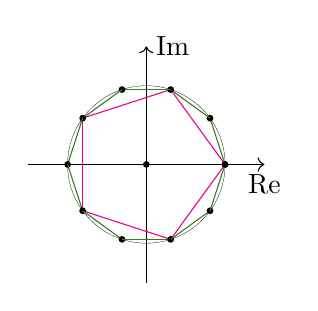
\begin{tikzpicture}[baseline=0]
			      \draw[->] (-1.5,0) -- (1.5,0) node[below] {Re};
			      \draw[->] (0,-1.5) -- (0,1.5) node[right] {Im};
			      \draw[ultra thin] (0,0) circle (1);
			      \filldraw[thin] (0,0) circle (1pt); % Added the origin
			      \foreach \x in {0,...,10} {
					      \filldraw (\x*360/10:1) circle (1pt);
					      \ifnum\x<10
						      \draw[OliveGreen] (\x*360/10:1) -- ({(\x+1)*360/10}:1);
					      \fi
					      \ifnum\x<5
						      \draw[magenta] (\x*360/5:1) -- ({(\x+1)*360/5}:1);
					      \fi
				      }
		      \end{tikzpicture}

		      $"G_5" \subseteq G_{10}$\\
		      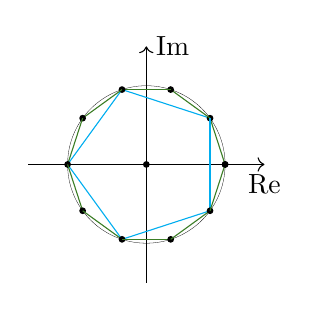
\begin{tikzpicture}[baseline=0]
			      \draw[->] (-1.5,0) -- (1.5,0) node[below] {Re};
			      \draw[->] (0,-1.5) -- (0,1.5) node[right] {Im};
			      \draw[ultra thin] (0,0) circle (1);
			      \filldraw[thin] (0,0) circle (1pt); % Added the origin
			      \foreach \x in {0,...,10} {
					      \filldraw (\x*360/10:1) circle (1pt);
					      \ifnum\x<10
						      \draw[OliveGreen] (\x*360/10:1) -- ({(\x+1)*360/10}:1);
					      \fi
					      \ifnum\x<5
						      \draw[cyan] ({\x*360/5+360/10}:1) -- ({(\x+1)*360/5+360/10}:1);
					      \fi
				      }
		      \end{tikzpicture}\\
	      \end{minipage}

	\item Calcular $w^{14} + w^{-8} + \conj w^4 + \conj{w^{-3}}$ para cada $w \en G_5$

	      \separadorCorto
	      \textit{Si} $w = 1$: \\
	      $w^{14} + w^{-8} + \conj w^4 + \conj{w^{-3}} = 4$

	      \textit{Si} $w \distinto 1$: \\
	      $w^{14} + w^{-8} + \conj w^4 + \conj{w^{-3}} =
		      w^4 + w^2 + w + w^3 =
		      \magenta{-1} + \ub{\magenta{1} + w + w^2 + w^3 + w^4}{= 0} = -1 $


\end{enumerate}
\newpage
%12
\ejercicio
\begin{enumerate}[label=\roman*)]
	\item Sea $w \en G_{36}$, $w^4 \distinto 1.$ Calcular $\sumatoria{k=7}{60}w^{4k}$

	      \separadorCorto
	      Sé que si $w \en G_{36} \entonces
		      \llave{l}{
			      w^{36} = 1 \\
			      \sumatoria{k=0}{35} w^k = 0
		      }$\\
	      Como $w^4 \distinto 1$ sé que $w \distinto \pm1$. Si no tendría que considerar casos particulares para la suma.\\

	      Si
	      $\sumatoria{k=7}{60}w^{4k} =
		      \ub{\sumatoria{k=7}{60}w^{4k} + \magenta{\sumatoria{k=0}{6}w^{4k}}}{\sumatoria{k=0}{60}w^{4k}}
		      - \magenta{\sumatoria{k=0}{6}w^{4k}} =
		      \sumatoria{k=0}{60}w^{4k} - \sumatoria{k=0}{6}w^{4k} =
		      \frac{(w^4)^{61} - 1}{w^4 - 1} - \frac{(w^4)^7 - 1}{w^4 - 1} =
		      \frac{(w^4)^{61} - (w^4)^7 }{w^4 - 1}\\
		      \flecha{$61 = 9\cdot6 + 7 $}[$w^36 = 1$]
		      \frac{((\ob{ \scriptstyle w^{36}}{=1})^6  \cdot (w^4)^7 - (w^4)^7 }{w^4 - 1}
		      \to$
	      \boxed{\sumatoria{k=7}{60}w^{4k} =0}

	\item Sea $w \en G_{11}$, $w \distinto 1.$ Calcular $\re\parentesis{\sumatoria{k=0}{60}w^k}$.

	      \separadorCorto
	      Sé que si $w \en G_{11} \entonces
		      \llave{l}{
			      w^{11} = 1 \\
			      \sumatoria{k=0}{10} w^k = 0\\
			      11 \text{ es impar} \entonces -1 \not\en G_{11}
		      }$\\
	      Como $w \distinto 1$ no calculo caso particular para la suma.
	      Me piden la parte real $ \flecha{uso} \re(z) = \frac{z + \conj z}{2}$.\\

	      Probé hacer la suma de Gauss como en el anterior, pero no llegué a nada, abro sumatoria y uso que $61 = 5 \cdot 11 +6$, porque hay 61 sumandos.\\

	      $\sumatoria{k=0}{60}w^k =
		      w^0 + \dots + w^{60} =
		      5 \cdot \ub{\ob{(w^0 + w^1 + \dots + w^9 + w^{10})}{=0}}{\text{\tiny agrupé usando: }w \en G^{11} \entonces w^k = w^{r_{11}(k)}} +
		      w^{55} + w^{56} + w^{57} + w^{58} + w^{59} + w^{60}=\\
		      = w^0 + w^1 + w^2 + w^3 + w^4 + w^5 \llamada{1}
	      $\\

	      También voy a usar que si $w \en G_{11} \entonces \conj w^k = w^{r_{11}(-k)}$\\
          $\re{\sumatoria{k=0}{60}w^k} = \frac{\sumatoria{k=0}{60}w^k +\sumatoria{k=0}{60}\conj w^k}{2} \stackrel{\llamada1}=
              \frac{w^0 + w^1 + w^2 + w^3 + w^4 + w^5 + \conj w^0 + \conj w^1 + \conj w^2 + \conj w^3 + \conj w^4 + \conj w^5}{2} =\\
              = \frac{w^0}{2} + \frac{\ob{w^1 + w^2 + w^3 + w^4 + w^5 + w^0 + w^{10} + w^9 + w^8 + w^7 + w^6}{\sumatoria{k=0}{10} w^k}}{2} =
              \frac{\ob{w^0}{1}}{2} + \frac{\ob{\sumatoria{k=0}{10} w^k}{= 0}}{2} = \frac{1}{2}
	      $
\end{enumerate}


%13
\ejercicio
Sea $w = e^{\frac{2\pi}{3}i}$ raíz cúbica de la unidad y sea $(z_n)_{n\en \naturales}$ la sucesión de números
complejos definida por:
\[
	z_1 = 1+w \quad \text{y} \quad z_{n+1} = \conj{1 + z_n^2},\, \paratodo n \en \naturales.
\]
Probar que para todo $n \en \naturales$ vale que
$z_n =
	\llave{ll}{
		e^{\frac{2\pi}{6}i}  & \text{si $n$ impar}\\
		e^{-\frac{2\pi}{6}i}  & \text{si $n$ par}
	}$. Concluir que $z_n \en G_6$ para todo $n \en \naturales$.

\separadorCorto
\begin{minipage}{0.75\textwidth}
	Hay que probar por inducción. Quiero probar:\\
	$p(n) :
		z_n =
		\llave{ll}{
			e^{\frac{2\pi}{6}i}  & \text{si $n$ impar}\\
			e^{-\frac{2\pi}{6}i}  & \text{si $n$ par}
		} \paratodo n \en \naturales\\
		\textit{Caso base: }\\
		\llave{l}{
          p(1) : z_1 = 1 + e^{\frac{2\pi}{3}i} = 1 -\frac{1}{2} + i \frac{\sqrt{3}}{2} = \frac{1}{2} + i \frac{\sqrt{3}}{2} =  e^{\frac{\pi}{3}i} \Tilde\\
			p(2) : z_2 = \conj{ 1 + z_1^2} = \conj{ 1 + e^{\frac{2\pi}{3}i} } = 1 + e^{-\frac{2\pi}{3}i} = e^{-\frac{\pi}{3}i} \Tilde
		}$\\

	\textit{Paso inductivo: }\\
	$\llave{l}{
			p(2k) : z_{2k} = e^{-\frac{\pi}{3}i} \ \text{Verdadero} \entonces p(2k+2) \  \text{¿Verdadero?}\\
			p(2k+1) : z_{2k+1} = e^{\frac{\pi}{3}i} \ \text{Verdadero} \entonces p(2k+3) \  \text{¿Verdadero?}
		}\\
		\llave{l}{
			z_{2k+2} = \conj{ 1 + z_{2k+1}^2 }
			\stackrel{HI}{\sisolosi} z_{2k+2} =
			\conj{ 1 + e^{\frac{2\pi}{3}i} } =
			\conj{ e^{\frac{\pi}{3}i} } =
			e^{-\frac{\pi}{3}i} \Tilde
			\\
			z_{2k+3} = \conj{ 1 + z_{2k+2}^2 }
			\stackrel{HI}{\sisolosi} z_{2k+3} =
			\conj{ 1 + e^{-\frac{2\pi}{3}i} } =
			\conj{ e^{-\frac{\pi}{3}i} } =
			e^{\frac{\pi}{3}i} \Tilde
		}$\\

	Dado que $p(1), p(2), p(2k),p(2k+1),p(2k+2),p(2k+3)$ resultaron ser verdaderas, entonces
	por el principio de inducción se concluye que $p(n)$ también lo es $\paratodo n \en \naturales$.\\
	Dado que la sucesión $z_n$   tiene solo 2 imágenes, para cualquier $n\en \naturales$ y teniendo en cuenta
    que $e^{-i\frac{2\pi}{6}} = e^{i\frac{2\pi}{6}\cdot 5} \en G_6\ \paratodo n \en \naturales$
\end{minipage}
\begin{minipage}{0.3\textwidth}
	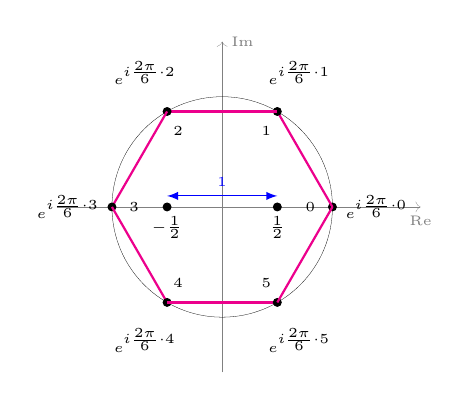
\begin{tikzpicture}[baseline=0,scale = 1.4, every node/.style={font=\tiny}]
		\draw[ultra thin,->,gray] (-1.5,0) -- (1.8,0) node[below] {Re};
		\draw[ultra thin,->,gray] (0,-1.5) -- (0,1.5) node[right] {Im};
		\draw[ultra thin] (0,0) circle (1);
		\filldraw[thin] (-.5,0) circle (1pt) node[below] {$-\frac{1}{2}$}; % Added the origin
		\filldraw[thin] (.5,0) circle (1pt) node[below] {$\frac{1}{2}$}; % Added the origin
		\draw[latex-latex, blue] (-.5,0.1) -- (0.5,0.1) node[midway, above]{ 1};
		\foreach \x in {0,...,5} {
				\filldraw (\x*360/6:1) circle (1pt) ;
				\filldraw (\x*360/6:0.8) node { $\x$};
                \filldraw (\x*360/6:1.4) node { $e^{i \frac{2\pi}{6} \cdot \x}$};
				\ifnum\x<6
					\draw[thick, magenta] (\x*360/6:1) -- ({(\x+1)*360/6}:1);
				\fi
				% \ifnum\x<3
				% 	\draw[thick, cyan] ({\x*360/3+360/3}:1) -- ({(\x+1)*360/3+360/3}:1);
				% \fi
			}
	\end{tikzpicture}
\end{minipage}
\red{corroborar con profes que no sea un delirio}


%14
\ejercicio
Se define en $\complejos - \set{0}$ la relación $\relacion$ dada por $z \relacion w \sisolosi z \conj w \en \reales_{>0}$.
\begin{enumerate}[label=\roman*)]
	\item Probar que $\relacion$ es una relación de equivalencia.
	\item Dibujar en le plano complejo la clase de equivalencia de $z = 1 + i$.
\end{enumerate}

\separadorCorto

\begin{enumerate}[label=\roman*)]
	\item Dado un $z = r e^{i\theta}$, tengo que $z\en \reales_{>0} \sisolosi
		      \re(z) > 0 \y \im(z) = 0 \sisolosi
		      r > 0 \y \theta = 2k\pi$ con $k \en \enteros$
	      \begin{itemize}
		      \item  \textit{Reflexividad: } $z = r e^{i\theta},\, z \relacion z = r^2 e^{2\theta i}$ por lo tanto
		            $z \relacion z \sisolosi 2\theta = 2 k\pi \sisolosi \theta = k\pi \Tilde$

		      \item  \textit{Simetría: }
		            $\llave{l}{
				            z \relacion w = r s  e^{(\theta -\varphi )i} \sisolosi \theta = 2k_1\pi + \varphi \Tilde\\
				            w \relacion z = r s  e^{(\varphi - \theta )i} \sisolosi \theta = -2k_2\pi + \varphi = 2k_3\pi + \varphi  \Tilde
			            }$

		      \item  \textit{Transitividad: }
		            $\llave{l}{
				            z \relacion w = r s  e^{(\theta - \varphi )i} \sisolosi \theta = 2k_1\pi + \varphi \\
				            w \relacion v = r t  e^{(\varphi - \alpha )i} \sisolosi \varphi = 2k_2\pi + \alpha \\
				            \entonces z \relacion v \sisolosi \theta =  2k_1\pi + \ub{\varphi}{2k_2\pi + \alpha} = 2\pi(k_1 + k_2) + \alpha = 2k_3\pi + \alpha \Tilde
			            }$\\
		            La relación $\relacion$ es de equivalencia.
	      \end{itemize}

	\item
	      \begin{minipage}{0.7\textwidth}
		      Tengo que el arg$( 1 + i) = \frac{\pi}{4}$. La clase  $\clase z$ estará formada por los $w \en \complejos$ tal que:
		      \boxed{ w \relacion z \sisolosi \text{arg}(w) = \frac{1}{4}\pi}
	      \end{minipage}
	      \begin{minipage}{0.3\textwidth}
		      \begin{tikzpicture}[baseline=0, scale = 2, every node/.style={font=\tiny}]
			      % \draw[help lines, dashed, step=0.25, ultra thin](-.5,-0.5) grid (1.5,1.5);

			      \draw[ultra thin,->,gray] (-.5,0) -- (1.5,0) node[below] {Re};
			      \draw[ultra thin,->,gray] (0,-.5) -- (0,1.5) node[right] {Im};
			      \draw[dotted, magenta, -latex] (0,0) -- (1.5,1.5) node[right] {$\clase{z}$};
			      % \draw[ultra thin] (0,0) circle (1);
			      \filldraw[thin] (1,1) circle (0.5pt) node[above] {$z$}; % Added the origin
			      \draw[thin] (0,0) circle (2pt); % Added the origin
			      \draw[thin, decorate,decoration={brace,amplitude=2pt,mirror,raise=1pt}] (0,0) -- (1,1) node[midway,below right] {$\sqrt{2}$} ;
		      \end{tikzpicture}
	      \end{minipage}
\end{enumerate}

%15
\ejercicio
Se define la siguiente relación $\relacion$ en $G_{20}$:
\[
	z\relacion w \sisolosi zw^9 \en G_2.
\]
\begin{enumerate}[label=\roman*)]
	\item Probar que $\relacion$ es una relación de equivalencia.
	\item Calcular la cantidad de elementos que hay en cada clase de equivalencia.
\end{enumerate}

\separadorCorto
\begin{enumerate}[label=\roman*)]
	\item
	      \textit{Reflexividad: }\\
	      $ z = e^{i\frac{1}{10}\pi k_z} \entonces
		      z \relacion z \sisolosi
		      e^{i\frac{1}{10}\pi k_z} \cdot e^{i\frac{9}{10}\pi k_z} =
		      e^{ik_z\pi } =
		      \llave{rl}{
			      1 & k_z \text{ par}\\
			      -1 & k_z \text{ impar}\\
		      } \Tilde
	      $\\

	      \textit{Simetría: }\\
	      $ z = e^{i\frac{1}{10}\pi k_z} \text{ y }  w = e^{i\frac{1}{10}\pi k_w} \en G_{20}.$

	      $\relacion$ es simétrica si:  $z \relacion w  \sisolosi w\relacion z\\
		      \llave{l}{
		      zw^9 = e^{i \frac{\pi}{10}(k_z + 9k_w)} \en G_2 \sii
		      \frac{1}{10}(k_z + 9k_w) = k \sii
		      k_z + 9k_w = 10k \sii
		      \congruencia{k_z}{-9k_w}{10} \sii
		      \congruencia{k_z}{k_w}{10} \\
		      \to \boxed{ z\relacion w  \sisolosi \congruencia{k_z}{k_w}{10}}\\

		      wz^9 = e^{i \frac{\pi}{10}(k_w + 9\magenta{k_z})} =
		      e^{i \frac{\pi}{10}(k_w + 9(\magenta{10k + k_w}))} =
				      e^{i \frac{\pi}{10}(90k + 10k_w)} =
				      e^{i (9k + k_w)\pi} =
				      e^{i\blue{k'}\pi}\\
			      }$\\
	      $\boxed{z \relacion w \sisolosi w \relacion z} \paratodo k,\,k_w \en \enteros \text{ con } \congruencia{k_z}{k_w}{10}\Tilde$\\

	      \textit{Transitividad: }\\
	      $ \llaves{l}{
			      z = e^{i\frac{1}{10}\pi k_z}\\
			      w = e^{i\frac{1}{10}\pi k_w}\\
			      y = e^{i\frac{1}{10}\pi k_y}
		      } \en G_{20}
		      \to
		      \relacion$ es transitiva si:  $z \relacion w  \text{ y } w\relacion y \entonces z \relacion y\\
		      \llaves{l}{
			      z \relacion w \sisolosi \congruencia{k_z}{k_w}{10} \llamada{1}\\
			      w \relacion y \sisolosi \congruencia{k_w}{k_y}{10} \llamada{2}
		      }\\
		      \to
		      zy^9 = e^{i \frac{\pi}{10}(\magenta{k_z} + 9k_y)} \stackrel{\llamada{1}}=
		      e^{i \frac{\pi}{10}(\magenta{10 k + k_w} + 9k_y)} \stackrel{\llamada{1}}=
		      e^{i \frac{\pi}{10}(10 k + 10k' + k_y + 9k_y)} =
		      e^{i (k + k' + k_y) \pi}  =
		      e^{i \blue{k''} \pi}
		      \\
		      \boxed{
			      \llaves{l}{
				      z \relacion w\\
				      w \relacion z
			      } \entonces z\relacion y}$

	\item $\# \clase{e^{i\frac{2\pi}{20} k}} = 2$ para algún $k \en \enteros / r_{20}(k) < 20$. Dada
	      la condición $\congruencia{k_z}{k_w}{10}$, solo hay 2 números que tienen misma cifra de unidad
	      entre 0 y 20. En el gráfico se ve que si $z\relacion w \entonces w = -z $
\end{enumerate}

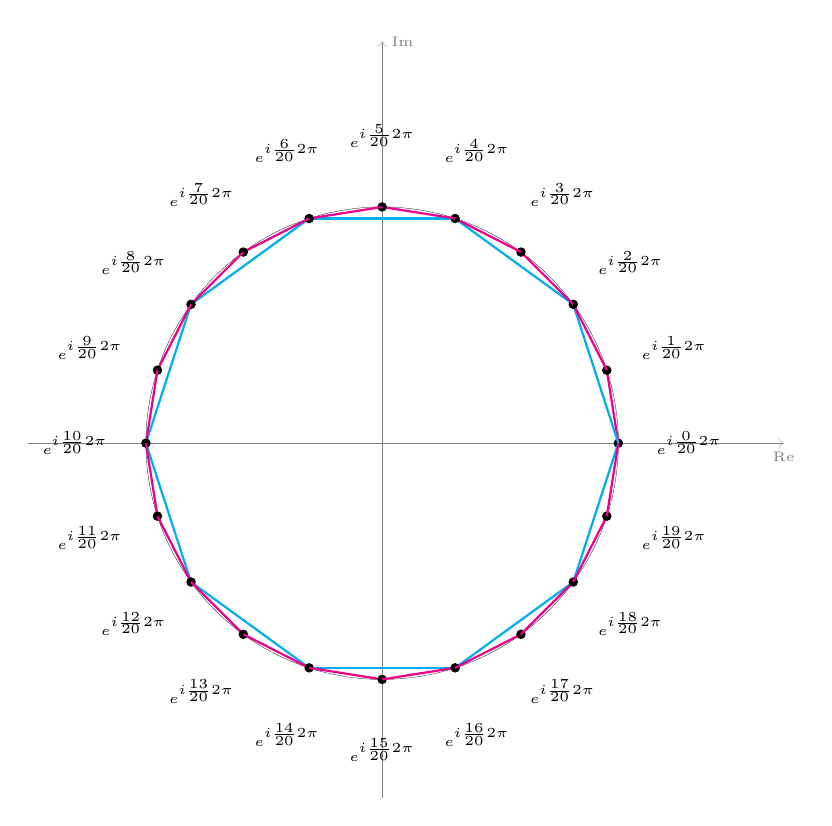
\begin{tikzpicture}[baseline=0,scale = 3, every node/.style={font=\tiny}]
	\draw[ultra thin,->,gray] (-1.5,0) -- (1.7,0) node[below] {Re};
	\draw[ultra thin,->,gray] (0,-1.5) -- (0,1.7) node[right] {Im};
	\draw[ultra thin] (0,0) circle (1);
	\foreach \x in {0,...,19} {
			\filldraw (\x*360/20:1) circle (0.5pt);
			\filldraw (\x*360/20:1.3) node { $e^{i\frac{\x}{20}2\pi}$};
			\ifnum\x<20
				\draw[thick, magenta] (\x*360/20:1) -- ({(\x+1)*360/20}:1);
			\fi
			\ifnum\x<10
				\draw[thick, cyan] (\x*360/10:1) -- ({(\x+1)*360/10}:1);
			\fi
		}
\end{tikzpicture}
\end{document}
